\begin{figure}[h!]
	\centering
	
	
	\tikzset{every picture/.style={line width=0.75pt}} %set default line width to 0.75pt        
	
	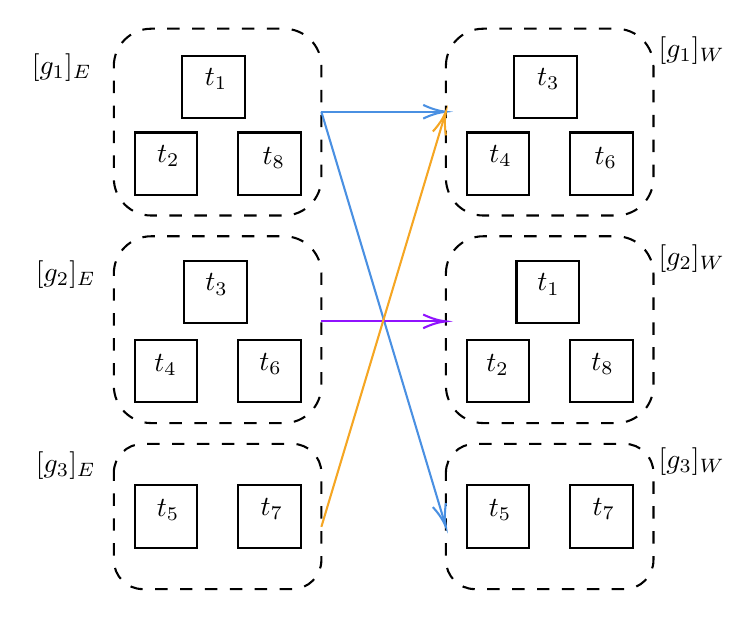
\begin{tikzpicture}[x=0.75pt,y=0.75pt,yscale=-1,xscale=1]
		%uncomment if require: \path (0,300); %set diagram left start at 0, and has height of 300
		
		%Shape: Square [id:dp9827031405699634] 
		\draw   (320,160) -- (350,160) -- (350,190) -- (320,190) -- cycle ;
		%Shape: Square [id:dp8023961227081475] 
		\draw   (370,230) -- (400,230) -- (400,260) -- (370,260) -- cycle ;
		%Shape: Square [id:dp03712561702321415] 
		\draw   (370,160) -- (400,160) -- (400,190) -- (370,190) -- cycle ;
		%Shape: Square [id:dp665252748842778] 
		\draw   (320,60) -- (350,60) -- (350,90) -- (320,90) -- cycle ;
		
		%Shape: Square [id:dp8558270957306437] 
		\draw   (343,23) -- (373,23) -- (373,53) -- (343,53) -- cycle ;
		%Shape: Square [id:dp7592436585314244] 
		\draw   (370,60) -- (400,60) -- (400,90) -- (370,90) -- cycle ;
		%Shape: Square [id:dp5096150167457512] 
		\draw   (320,230) -- (350,230) -- (350,260) -- (320,260) -- cycle ;
		%Shape: Square [id:dp468896653565648] 
		\draw   (344,122) -- (374,122) -- (374,152) -- (344,152) -- cycle ;
		%Shape: Square [id:dp5959228737950086] 
		\draw   (160,160) -- (190,160) -- (190,190) -- (160,190) -- cycle ;
		%Shape: Square [id:dp4137689515105887] 
		\draw   (210,230) -- (240,230) -- (240,260) -- (210,260) -- cycle ;
		%Shape: Square [id:dp2890656867000987] 
		\draw   (210,160) -- (240,160) -- (240,190) -- (210,190) -- cycle ;
		%Shape: Square [id:dp2222867301895708] 
		\draw   (160,60) -- (190,60) -- (190,90) -- (160,90) -- cycle ;
		
		%Shape: Square [id:dp9529971943334293] 
		\draw   (183,23) -- (213,23) -- (213,53) -- (183,53) -- cycle ;
		%Shape: Square [id:dp3186523365427516] 
		\draw   (210,60) -- (240,60) -- (240,90) -- (210,90) -- cycle ;
		%Shape: Square [id:dp6108775427683606] 
		\draw   (160,230) -- (190,230) -- (190,260) -- (160,260) -- cycle ;
		%Shape: Square [id:dp4159406011644433] 
		\draw   (184,122) -- (214,122) -- (214,152) -- (184,152) -- cycle ;
		%Rounded Rect [id:dp6633339374263201] 
		\draw  [dash pattern={on 4.5pt off 4.5pt}] (150,28) .. controls (150,18.06) and (158.06,10) .. (168,10) -- (232,10) .. controls (241.94,10) and (250,18.06) .. (250,28) -- (250,82) .. controls (250,91.94) and (241.94,100) .. (232,100) -- (168,100) .. controls (158.06,100) and (150,91.94) .. (150,82) -- cycle ;
		%Rounded Rect [id:dp07771024867524312] 
		\draw  [dash pattern={on 4.5pt off 4.5pt}] (150,128) .. controls (150,118.06) and (158.06,110) .. (168,110) -- (232,110) .. controls (241.94,110) and (250,118.06) .. (250,128) -- (250,182) .. controls (250,191.94) and (241.94,200) .. (232,200) -- (168,200) .. controls (158.06,200) and (150,191.94) .. (150,182) -- cycle ;
		%Rounded Rect [id:dp03141626075041437] 
		\draw  [dash pattern={on 4.5pt off 4.5pt}] (150,224) .. controls (150,216.27) and (156.27,210) .. (164,210) -- (236,210) .. controls (243.73,210) and (250,216.27) .. (250,224) -- (250,266) .. controls (250,273.73) and (243.73,280) .. (236,280) -- (164,280) .. controls (156.27,280) and (150,273.73) .. (150,266) -- cycle ;
		%Rounded Rect [id:dp5622046683031108] 
		\draw  [dash pattern={on 4.5pt off 4.5pt}] (310,28) .. controls (310,18.06) and (318.06,10) .. (328,10) -- (392,10) .. controls (401.94,10) and (410,18.06) .. (410,28) -- (410,82) .. controls (410,91.94) and (401.94,100) .. (392,100) -- (328,100) .. controls (318.06,100) and (310,91.94) .. (310,82) -- cycle ;
		%Rounded Rect [id:dp20845445372702165] 
		\draw  [dash pattern={on 4.5pt off 4.5pt}] (310,128) .. controls (310,118.06) and (318.06,110) .. (328,110) -- (392,110) .. controls (401.94,110) and (410,118.06) .. (410,128) -- (410,182) .. controls (410,191.94) and (401.94,200) .. (392,200) -- (328,200) .. controls (318.06,200) and (310,191.94) .. (310,182) -- cycle ;
		%Rounded Rect [id:dp061768139424575264] 
		\draw  [dash pattern={on 4.5pt off 4.5pt}] (310,224) .. controls (310,216.27) and (316.27,210) .. (324,210) -- (396,210) .. controls (403.73,210) and (410,216.27) .. (410,224) -- (410,266) .. controls (410,273.73) and (403.73,280) .. (396,280) -- (324,280) .. controls (316.27,280) and (310,273.73) .. (310,266) -- cycle ;
		%Straight Lines [id:da06878187278722059] 
		\draw [color={rgb, 255:red, 74; green, 144; blue, 226 }  ,draw opacity=1 ]   (250,50) -- (308,50) ;
		\draw [shift={(310,50)}, rotate = 180] [color={rgb, 255:red, 74; green, 144; blue, 226 }  ,draw opacity=1 ][line width=0.75]    (10.93,-3.29) .. controls (6.95,-1.4) and (3.31,-0.3) .. (0,0) .. controls (3.31,0.3) and (6.95,1.4) .. (10.93,3.29)   ;
		%Straight Lines [id:da03355516067793607] 
		\draw [color={rgb, 255:red, 74; green, 144; blue, 226 }  ,draw opacity=1 ]   (250,50) -- (309.43,248.08) ;
		\draw [shift={(310,250)}, rotate = 253.3] [color={rgb, 255:red, 74; green, 144; blue, 226 }  ,draw opacity=1 ][line width=0.75]    (10.93,-3.29) .. controls (6.95,-1.4) and (3.31,-0.3) .. (0,0) .. controls (3.31,0.3) and (6.95,1.4) .. (10.93,3.29)   ;
		%Straight Lines [id:da18343296273423393] 
		\draw [color={rgb, 255:red, 144; green, 19; blue, 254 }  ,draw opacity=1 ]   (250,151) -- (308,151) ;
		\draw [shift={(310,151)}, rotate = 180] [color={rgb, 255:red, 144; green, 19; blue, 254 }  ,draw opacity=1 ][line width=0.75]    (10.93,-3.29) .. controls (6.95,-1.4) and (3.31,-0.3) .. (0,0) .. controls (3.31,0.3) and (6.95,1.4) .. (10.93,3.29)   ;
		%Straight Lines [id:da707149216624745] 
		\draw [color={rgb, 255:red, 245; green, 166; blue, 35 }  ,draw opacity=1 ]   (250,250) -- (309.43,51.92) ;
		\draw [shift={(310,50)}, rotate = 106.7] [color={rgb, 255:red, 245; green, 166; blue, 35 }  ,draw opacity=1 ][line width=0.75]    (10.93,-3.29) .. controls (6.95,-1.4) and (3.31,-0.3) .. (0,0) .. controls (3.31,0.3) and (6.95,1.4) .. (10.93,3.29)   ;
		
		% Text Node
		\draw (328,165.4) node [anchor=north west][inner sep=0.75pt]    {$t_{2}$};
		% Text Node
		\draw (378.6,165) node [anchor=north west][inner sep=0.75pt]    {$t_{8}$};
		% Text Node
		\draw (352.4,27.8) node [anchor=north west][inner sep=0.75pt]    {$t_{3}$};
		% Text Node
		\draw (379.2,235) node [anchor=north west][inner sep=0.75pt]    {$t_{7}$};
		% Text Node
		\draw (380.2,65.8) node [anchor=north west][inner sep=0.75pt]    {$t_{6}$};
		% Text Node
		\draw (329.2,235.2) node [anchor=north west][inner sep=0.75pt]    {$t_{5}$};
		% Text Node
		\draw (352.6,126.6) node [anchor=north west][inner sep=0.75pt]    {$t_{1}$};
		% Text Node
		\draw (329.4,64.6) node [anchor=north west][inner sep=0.75pt]    {$t_{4}$};
		% Text Node
		\draw (168,165.4) node [anchor=north west][inner sep=0.75pt]    {$t_{4}$};
		% Text Node
		\draw (218.6,165) node [anchor=north west][inner sep=0.75pt]    {$t_{6}$};
		% Text Node
		\draw (192.4,27.8) node [anchor=north west][inner sep=0.75pt]    {$t_{1}$};
		% Text Node
		\draw (219.2,235) node [anchor=north west][inner sep=0.75pt]    {$t_{7}$};
		% Text Node
		\draw (220.2,65.8) node [anchor=north west][inner sep=0.75pt]    {$t_{8}$};
		% Text Node
		\draw (169.2,235.2) node [anchor=north west][inner sep=0.75pt]    {$t_{5}$};
		% Text Node
		\draw (192.6,126.6) node [anchor=north west][inner sep=0.75pt]    {$t_{3}$};
		% Text Node
		\draw (169.4,64.6) node [anchor=north west][inner sep=0.75pt]    {$t_{2}$};
		% Text Node
		\draw (109,20.4) node [anchor=north west][inner sep=0.75pt]    {$[ g_{1}]_{E}$};
		% Text Node
		\draw (111,120.4) node [anchor=north west][inner sep=0.75pt]    {$[ g_{2}]_{E}$};
		% Text Node
		\draw (111,212.4) node [anchor=north west][inner sep=0.75pt]    {$[ g_{3}]_{E}$};
		% Text Node
		\draw (411,12.4) node [anchor=north west][inner sep=0.75pt]    {$[ g_{1}]_{W}$};
		% Text Node
		\draw (411,112.4) node [anchor=north west][inner sep=0.75pt]    {$[ g_{2}]_{W}$};
		% Text Node
		\draw (411,210.4) node [anchor=north west][inner sep=0.75pt]    {$[ g_{3}]_{W}$};
		
		
	\end{tikzpicture}
\end{figure}